\chapter{Introduzione al calcolo numerico}

Grazie al costante sviluppo dei computers negli scorsi decenni, la comunità scientifica ha avuto modo di usufruire di strumenti di calcolo sempre più precisi e complessi, necessari per risolvere alcuni problemi di vario tipo. Questo sviluppo ha visto anche un cospicuo interesse verso i metodi di calcolo numerico, che permettono di risolvere in modo non-analitico problemi specifici che non sarebbero, altrimenti, risolvibili. Infatti, seppur non esista sempre una soluzione analitica, \textbf{esiste sempre una soluzione numerica} per un modello matematico \textbf{ben posto} e \textbf{condizionato}, che assuma tuttavia certe assunzioni del corrispondente modello fisico.
\nl
La realtà infatti non è sempre modellabile attraverso semplici formule fisiche: a volte ci sono parecchie variabili da tenere in conto quando si cerca di risolvere un problema, e non è sempre plausibile considerare tutte queste variabili assieme, soprattutto se il problema va risolto senza l'assistenza di un calcolatore. Consideriamo il seguente esempio: un giocatore di golf colpisce una pallina con una certa velocità $U$, e noi vogliamo sapere per quale angolo $\alpha$ la distanza che verrebbe percorsa dalla pallina da golf sarebbe massima prima che quest'ultima tocchi terra.
\nl
Grazie alla seconda legge di Newton, possiamo calcolare la distanza percorsa dalla pallina, e se trascurassimo la resistenza dell'aria sarebbe abbastanza semplice trovare la soluzione analitica. Tuttavia, considerando questa resistenza, le equazioni del moto si complicano notevolmente, e determinare la soluzione analitica diventa ora impossibile. Tuttavia, la soluzione numerica rimane calcolabile attraverso l'impiego di metodi numerici adatti.
\nl
È comunque importante considerare anche il tipo di modello utilizzato: in base al modello matematico di partenza e al metodo utilizzato, si possono ottenere risultati diversi. L'importante è saper scegliere il metodo giusto e l'approssimazione migliore del modello.
\nl
Per il calcolo numerico, la risoluzione di un problema avviene attraverso i seguenti steps:
\begin{itemize}
    \item formulare un \textbf{modello matematico} in base al problema dato, che diventi uno schema per definire il metodo numerico e l'algoritmo di soluzione;
    \item scegliere un \textbf{metodo numerico} che aiuti nella risoluzione del problema;
    \item definire un \textbf{algoritmo} che porti alla soluzione desiderata;
    \item analizzare la \textbf{soluzione numerica} e interpretarla, capendo se quest'ultima sia una valida soluzione o meno. Si dice che una soluzione numerica sia \textbf{accettabile} se e solo se sia possibile \textbf{stimare gli errori} che accompagnano la soluzione stessa.
\end{itemize}

\section{Errori di approssimazione}

Quando si calcola una soluzione numerica, ci sono varie, possibili fonti di errori che possono condizionare il risultato finale. È possibile avere errori di \textbf{misura} (dati dalla precisione dello strumento), \textbf{inerenti} (creati da un'eccessiva semplificazione del modello reale), di \textbf{troncamento} (generati da una discretizzazione del risultato, generalmente presenti quando si usano metodi numerici che richiedono convergenza), e di \textbf{arrotondamento} (creati dalla macchina che performa i calcoli, in quando la precisione è sempre limitata).
\nl
Ogni computer dispone di un sistema numerico piuttosto primitivo: questo infatti dispone di un sistema \textbf{finito} di numeri, la cui lunghezza è anch'essa \textbf{finita}. Se normalmente, in campi analitici, siamo abituati a pensare con un insieme di numeri infinito (come quello dei numeri reali, $\mathbb{R}$), con i computer, quando si performano calcoli di analisi numerica, si considera un insieme ristretto, detto dei \textbf{numeri macchina} $\mathbb{F}$. Consideriamo ad esempio alcune delle costanti più famose nel mondo matematico: $\pi$, $e$ e $\sqrt{2}$. Noi sappiamo che questi numeri sono irrazionali, e che si espandono all'infinito. Proviamo a chiedere a una macchina di dirci quali sono questi numeri. Eseguendo il seguente script di Python, otterremo il seguente risultato:

\begin{codeblock}{Rounding.py}
    \begin{lstlisting}[language = Python]
import numpy as np
from math import sqrt

print(np.pi, np.e, sqrt(2), sep="\n")\end{lstlisting}
    \vspace{11pt}
    \begin{tcolorbox}[colback = black!95!Periwinkle!90]
        \begin{lstlisting}[style = notexterm]
Out[1]: 3.141592653589793
        2.718281828459045
        1.4142135623730951\end{lstlisting}
    \end{tcolorbox}
\end{codeblock}

Noi sappiamo che in realtà questi numeri si estendono molto più in profondità di quello che ci ha ritornato Python. Infatti:
\begin{itemize}
    \item $\pi = 3,1415926535897932384626433...$;
    \item $e = 2,71828182845904523536...$;
    \item $\sqrt{2} = 1,4142135623730950488...$
\end{itemize}

Qua notiamo già uno dei primi errori che si incontra quando si usa un calcolatore: i numeri sono \textbf{arrotondati} ad una certa cifra. L'arrotondamento genera spesso qualche tipo di errore, ma è necessario che i numeri subiscano una procedura di arrotondamento prima di poter essere usati da un calcolatore, poiché altrimenti non entrerebbero nella memoria di quest'ultimo, che ricordiamo essere limitata.

\begin{definition}{Errore di arrotondamento}
    Definitiamo l'\textbf{errore di arrotondamento} come la \textbf{differenza} tra il \textbf{numero reale} $x \in \mathbb{R}$ e il \textbf{numero macchina} $m \in \mathbb{F}$ corrispondente:
    \[ e_\text{arr} = x - m \]
\end{definition}

Se un calcolatore approssima tutti i numeri alla $D$esima cifra decimale, allora diciamo che l'errore di arrotondamento è compreso nell'\textbf{intervallo} $[-0,5 \cdot 10^{-D}, \; +0,5 \cdot 10^{-D}]$.
\nl
Riguardo lo scopo di queste note: MATLAB verrà usato durante il corso per implementare certi metodi numerici. Tale linguaggio di programmazione lavora con 15 cifre decimali significative. Fino a quando non verrà introdotto MATLAB tuttavia, verrà usato Python, che ne usa fino a 17 (anche se negli esempi precedenti $\pi$ e $e$ hanno usato solo 15 cifre, probabilmente a causa del pacchetto \verb|numpy|).
\nl
Consideriamo un esempio per comprendere l'importanza degli errori di arrotondamento:
\begin{example}
    Si considerino le due funzioni seguenti, che sono algebricamente equivalenti:
    \[ q_1(x) \eq (x - 1)^7 \quad \quad q_2(x) \eq x^7 - 7x^6 + 21x^5 - 35x^4 + 35x^3 - 21x^2 + 7x - 1 \]

    Vogliamo calcolare il valore numerico di $q_1(x)$ e $q_2(x)$ con due valori di $x$, ovverosia $1$ e $1,0001$, e confrontare il loro valore esatto con l'errore di arrotondamento. Vogliamo inoltre usare una macchina che lavori con 15 cifre significative. Usando il seguente script in Python, possiamo ottenere i nostri risultati:
    \begin{codeblock}{ApproxExample.py}
        \begin{lstlisting}[language = Python, numbers = none]
from math import pow

def q1(x) -> float:
    return (x - 1) ** 7

def q2(x) -> float:
    return pow(x, 7) - 7 * pow(x, 6) + 21 * pow(x, 5) \
        - 35 * pow(x, 4) + 35 * pow(x, 3) - 21 * pow(x, 2) + 7 * x - 1

def rounding_error(real, machine) -> float:
    return float(real) - float(machine)

# La lista contiene tuple del tipo (x, valore_reale)
for i, expect in [(1, 0), (1.0001, 10**(-28))]:
    # Approssimazione del numero alla 10a cifra decimale
    res1, res2 = "{0:.10g}".format(q1(i)), "{0:.10g}".format(q2(i))
    err1, err2 = rounding_error(expect, res1), rounding_error(expect, res2)
    print(f"With x = {i}, expect {expect}\nQ1 = {res1} | E1 = {err1}\nQ2 = {res2} | E2 = {err2}\n")\end{lstlisting}
        \nl
        \begin{tcolorbox}[colback = black!95!Periwinkle!90]
            \begin{lstlisting}[style = notexterm]
Out[1]: With x = 1, expect 0
        Q1 = 0 | E1 = 0.0
        Q2 = 0 | E2 = 0.0

        With x = 1.0001, expect 1e-28
        Q1 = 1e-28 | E1 = 0.0
        Q2 = 1.776356839e-15 | E2 = -1.7763568389999e-15\end{lstlisting}
        \end{tcolorbox}
    \end{codeblock}

    Come possiamo notare dall'output dello script, con $x = 1$ non c'è alcuna differenza tra $q_1(x)$ e $q_2(x)$, ma con $x = 1,0001$ iniziano ad esserci le prime differenze. Infatti, nel secondo caso abbiamo un errore di arrotondamento di circa $-1,78 \cdot 10^{-15}$. Questo semplice esempio dimostra come due quantità che sono algebricamente uguali possono in realtà portare a due risultati numerici completamente diversi.
    \nl
    Questo comportamento può essere inoltre osservato attraverso il seguente grafico:
    \begin{center}
        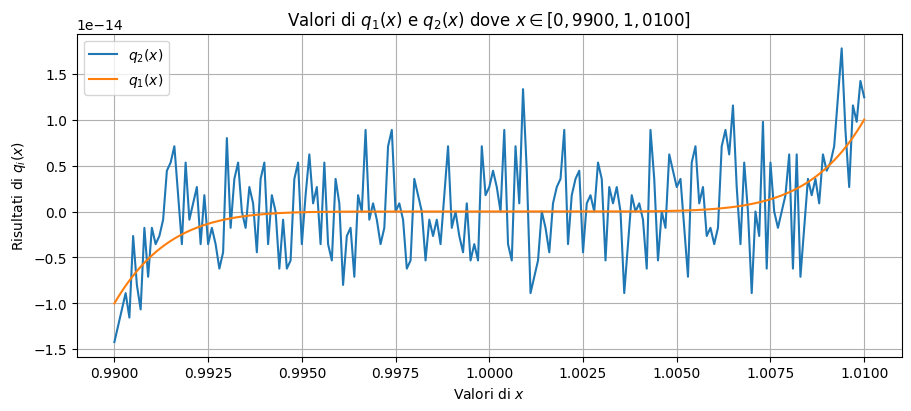
\includegraphics[width = \linewidth]{assets/image-001.png}
    \end{center}
\end{example}

